\svnid{$Id$}
\chapter{Nitric Oxide Reduction in \Nm{}}
\label{chap:noreduction}
\section{Aerobic Nitric Oxide Reduction}
\subsection{Introduction}
The next dataset I used in my iterative approach to parameter estimation was of one of aerobic oxygen reduction interrupted by the addition of Nitric Oxide. This dataset is the next most complicated after aerobic oxygen reduction as it introduces the nitric oxide reduction pathway. The portions of the ETC relating to Nitric Oxide reduction are shown graphically in Figure \ref{fig:no_resp_chain}. However this pathway cannot be isolated \textit{in vivo} as \Nm{} is incapable of completely anaerobic respiration therefore the required parts of the model are actually those from Chapter \ref{chap:oxygenreduction} and those in Figure \ref{fig:no_resp_chain}.
\begin{figure}[tbp]
  \centering
    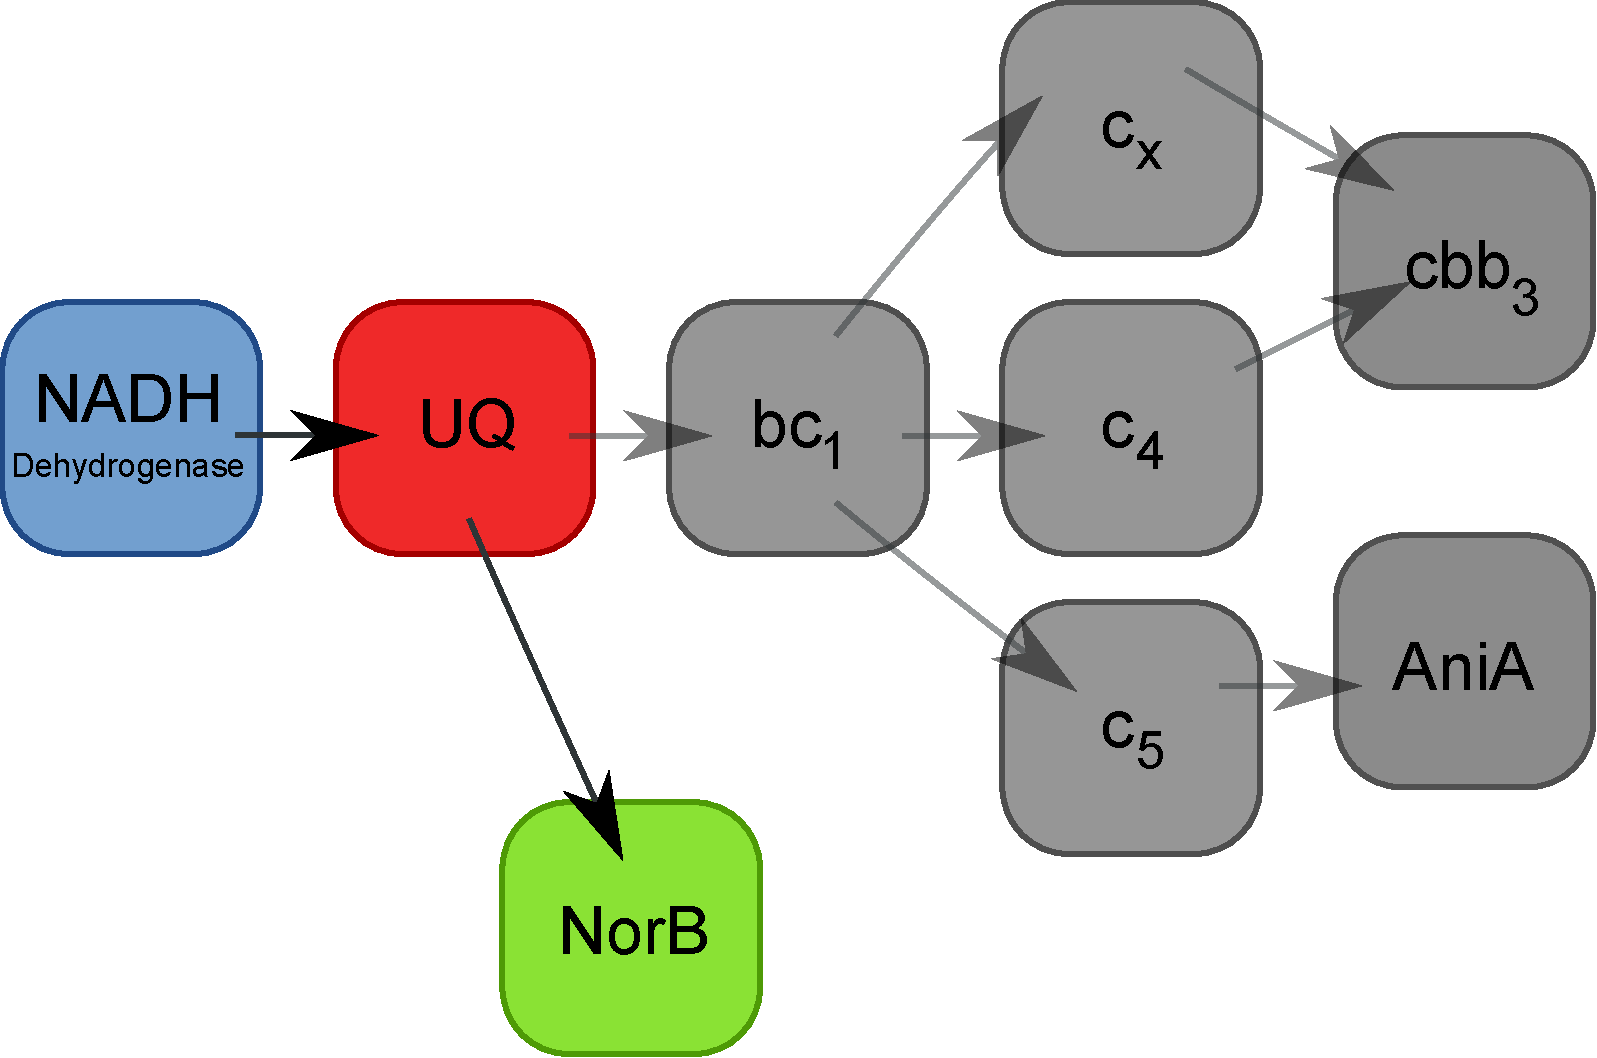
\includegraphics[width=14cm]{06-noreduction/data/no_resp_chain.pdf}
    \caption[Nitric oxide reducing electron transport chain of \Nm{}]{{\bf Nitric oxide reducing electron transport chain of \Nm{}.} This shows the complete electron transport chain of \Nsm{} with the components irrelevant to nitric oxide reduction greyed out.
  \label{fig:no_resp_chain}}
\end{figure}
The equations that describe this portion of the ETC are:
\begin{eqnarray*}
\frac{d[O_2]}{dt} & = & \beta(1-[O_2]/K_O) - k_{1}[C_a][O_2]\\
\frac{d[Q_a]}{dt} & = & g([Q] - [Q_a]) - l_3[Q_a]([B] - [B_a]) - f[Q_a]([X]-[X_a])\\
\frac{d[X_a]}{dt} & = & -k_3([C] - [C_a] - [C_X])[X_a]  - m_3([A] - [A_a])[X_a] + f[Q_a]([X]-[X_a])\\
\frac{d[C_a]}{dt} & = & k_3([C] - [C_a] - [C_X])[X_a] - k_{1}[C_a][O_2] - k_5[C_a][NO]\\
\frac{d[NO]}{dt} & = & m_{1}[NO_2^-][A_a] - l_1[NO][B_a] - k_5[C_a][NO] + k_6 [C_X] - \gamma[NO]\\
\frac{d[C_X]}{dt} & = & k_5[C_a][NO] - k_6 [C_X]\\
\frac{d[B_a]}{dt} & = & l_3[Q_a]([B] - [B_a]) - l_1[NO][B_a]
\end{eqnarray*}
These equations describe the change in concentration of Nitric Oxide over time, which is the experimentally observable value (in addition to the afore modelled oxygen). Also being modelled was the change in concentration of inhibited \cbbthree{} and the reduction state of NorB. This portion of the model involved 24 parameters and variables which I needed to estimate. This number includes the 13 values already estimated in Chapter \ref{chap:oxygenreduction}.
\subsection{Experimental Results}
Generation of nitric oxygen reduction datasets required the growth of MC58 (wild type \Nsm{}) in aerobic conditions until mid log-phase growth had been achieved. This corresponds to an $OD_{600}$ of 0.3-0.9 and usually required an incubation period of roughly 3 hours. Once the required cell density had been obtained, I transferred the culture to the oxygen electrode chamber and recorded the oxygen and nitric oxide concentrations as the culture respired. To model nitric oxide reduction required that I add nitric oxide solution to the culture while it is respiring aerobically. Part-way through aerobic respiration I added nitric oxide solution to various final concentrations at $\approx 5~\mu$M and the culture then left to respire nitric oxide. An example dataset showing the effect of addition of nitric oxide to an aerobically respiring culture is shown in Figures \ref{fig:nodata}, \ref{fig:nodata1} \& \ref{fig:nodata2}.

\begin{figure}[tbp]
 \centering
 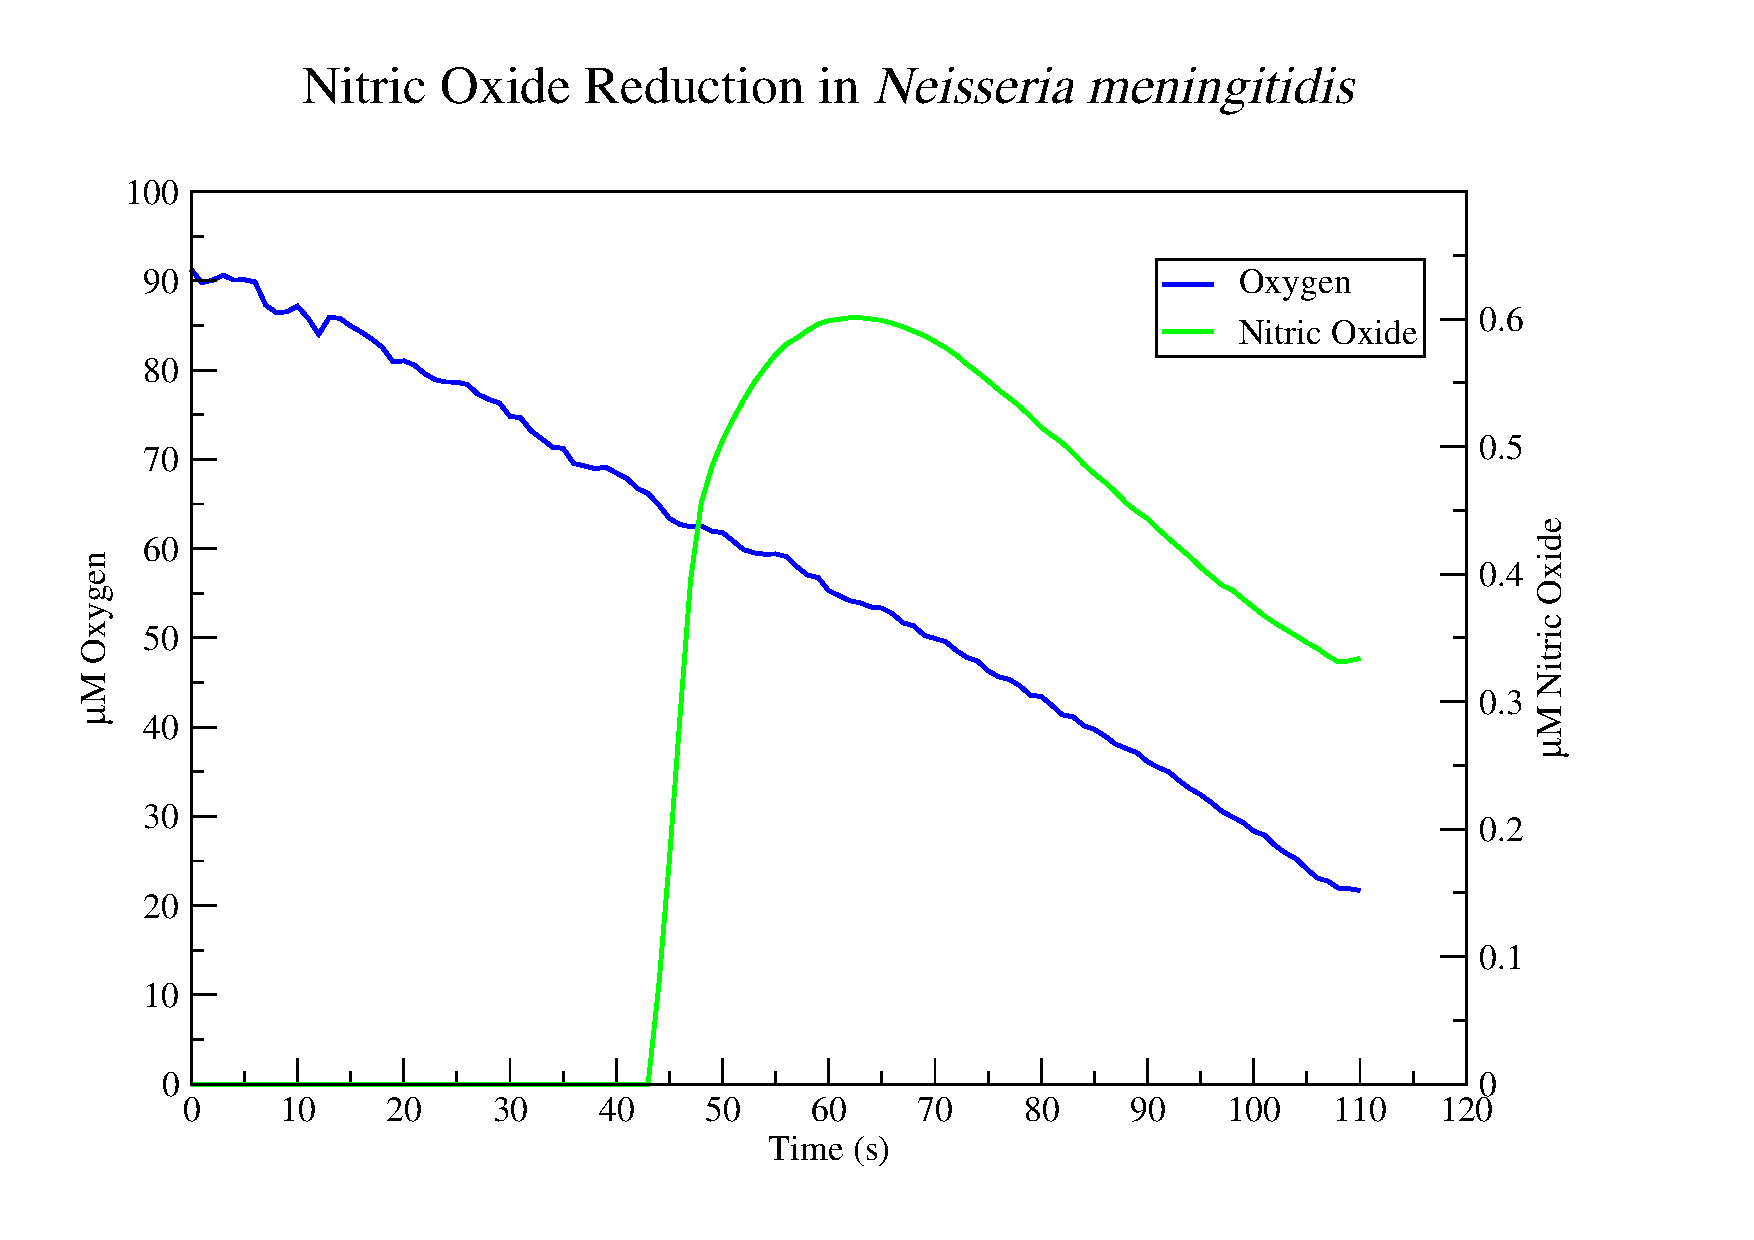
\includegraphics[height=10cm, trim=2cm 1cm 4cm 1cm]{./06-noreduction/data/aer-no-data1.pdf}
 % nosim.eps: 0x0 pixel, 300dpi, 0.00x0.00 cm, bb=0 0 794 595
 \caption[{Nitric Oxide Reduction in \textit{Neisseria meningitidis}.}]{{\bf Nitric Oxide Reduction in \textit{Neisseria meningitidis}.} This dataset shows the effect on rate of oxygen reduction as a small amount of nitric oxide is introduced to the system.}
 \label{fig:nodata1}
\end{figure}
The dataset in Figure \ref{fig:nodata1} shows very little change in the rate of oxygen reduction (it is in fact somewhere around a 3\% reduction in rate) when a small amount of nitric oxide is added. The observed removal of nitric oxide is due primarily to diffusion although there may also be some preliminary (as the culture has not been primed with nitric oxide) nitric oxide reductase activity.

\begin{figure}[tbp]
 \centering
 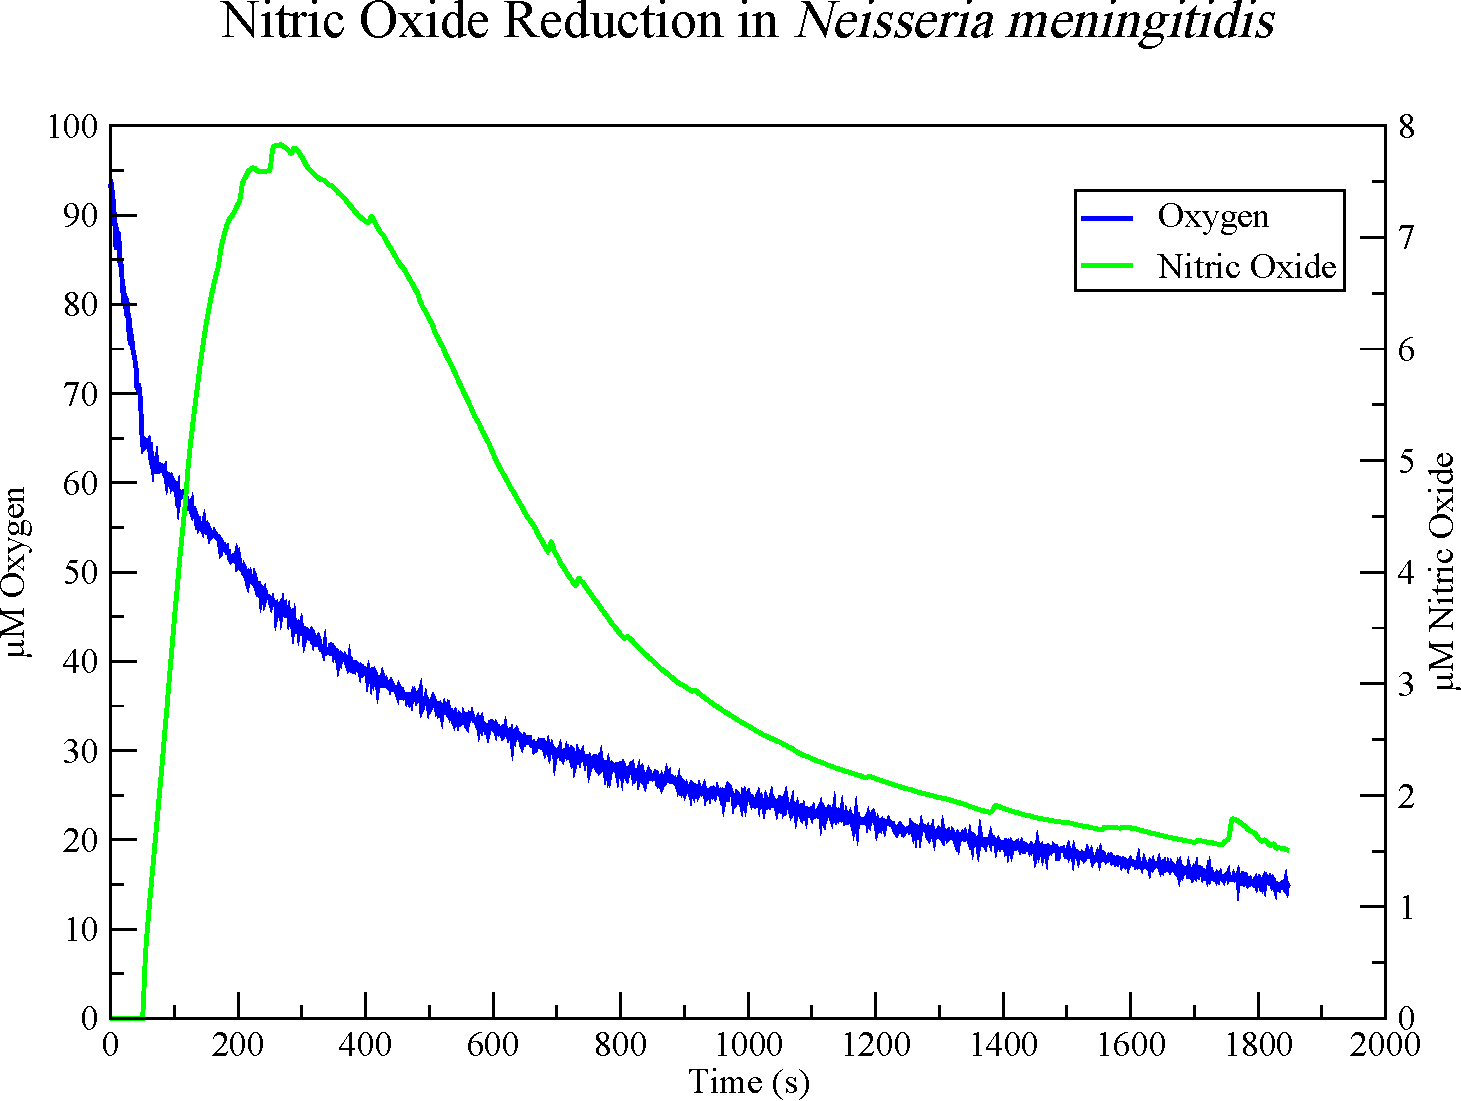
\includegraphics[height=10cm, trim=2cm 1cm 4cm 1cm]{./06-noreduction/data/aer-no-data2.pdf}
 % nosim.eps: 0x0 pixel, 300dpi, 0.00x0.00 cm, bb=0 0 794 595
 \caption[{Nitric Oxide Reduction in \textit{Neisseria meningitidis}.}]{{\bf Nitric Oxide Reduction in \textit{Neisseria meningitidis}.} This dataset shows the effect on rate of oxygen reduction as a larger amount of nitric oxide is introduced to the system.}
 \label{fig:nodata2}
\end{figure}
The dataset in Figure \ref{fig:nodata2} shows a larger change in the rate of oxygen reduction than that of Figure \ref{fig:nodata1} when a larger amount of nitric oxide is introduced. Again the removal of nitric oxide will primarily be due to diffusion, although now at higher concentrations more nitric oxide will interact with \cbbthree{} temporarily inhibiting it. This inhibition causes the reduction in oxidase activity, and the sequestering of NO by \cbbthree{} also causes some of the visible reduction in nitric oxide concentration. The time-scale over which the nitric oxide disappears strongly suggests that it is not due to nitric oxide reductase activity. It may also be possible that at this concentration of nitric oxide some \cbbthree{} may have been permanently inhibited as mentioned in Chapters \ref{chap:intro} \& \ref{chap:model}.

\begin{figure}[tbp]
 \centering
 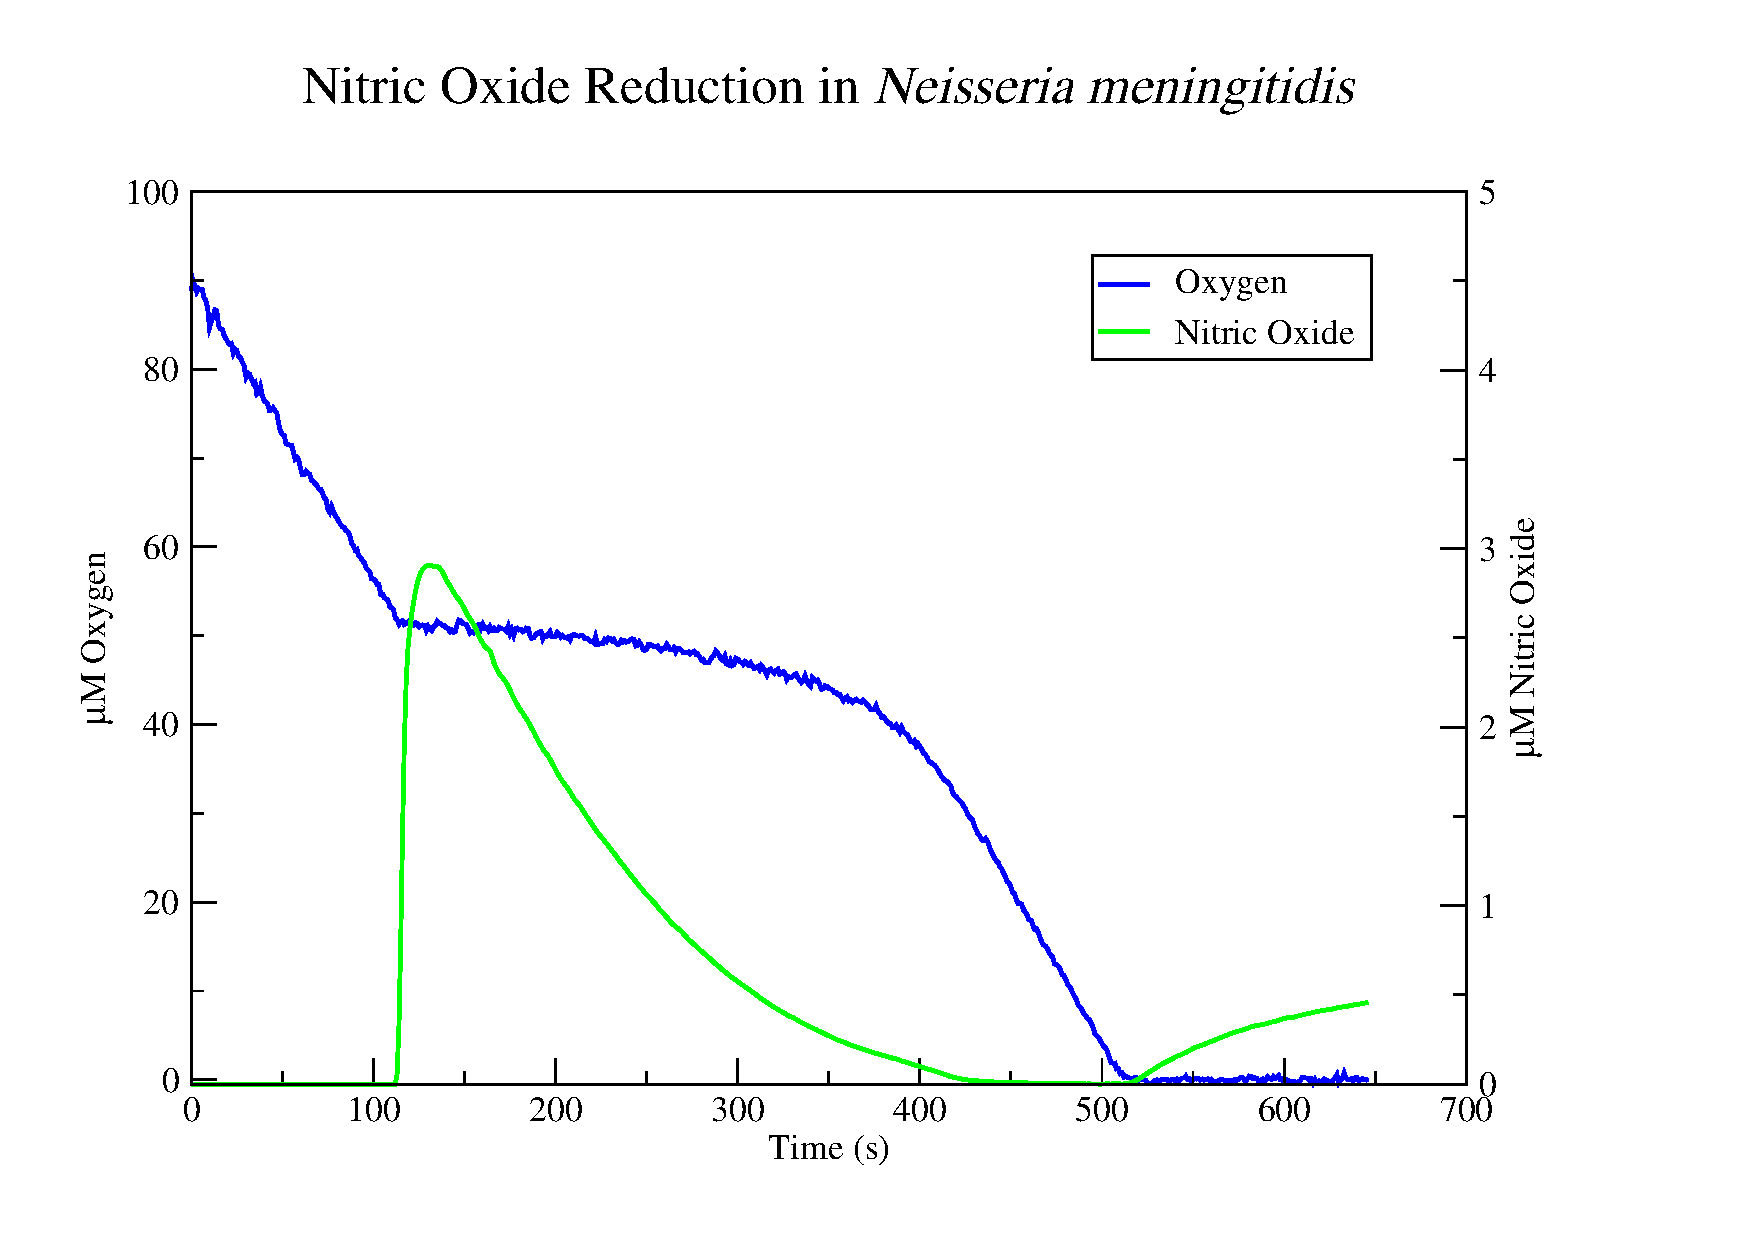
\includegraphics[height=10cm, trim=2cm 1cm 4cm 1cm]{./06-noreduction/data/aer-no-data.pdf}
 % nosim.eps: 0x0 pixel, 300dpi, 0.00x0.00 cm, bb=0 0 794 595
 \caption[{Nitric Oxide Reduction in \textit{Neisseria meningitidis}.}]{{\bf Nitric Oxide Reduction in \textit{Neisseria meningitidis}.} This dataset shows the effect on rate of oxygen reduction as nitric oxide is introduced to the system which appears to have been primed for nitric oxide reduction.}
 \label{fig:nodata}
\end{figure}
The dataset in Figure \ref{fig:nodata} appears to show a system that is partially primed for microaerobic respiration. In this case there is a small amount of NorB (nitric oxide reductase) present. Initially the oxygen reduction is carried out in exactly the same manner as in Chapter \ref{chap:oxygenreduction}. Upon addition of nitric oxide, oxygen respiration slows and almost stops as a result of competition for electrons between \cbbthree{} and NorB, and the direct chemical inhibition of \cbbthree{} by NO. Nitric oxide starts being removed as a combination of diffusion (although this rate will be low as shown in the previous two datasets) and reduction via NorB. Once the NO has been removed from the system oxygen reduction resumes at almost the same rate as before and still has the same high affinity feature as the oxygen reduction datasets in Chapter \ref{chap:oxygenreduction}.
\subsubsection{Prior Probability Distributions}
The prior probability distributions used for parameter estimation of these datasets were a combination of the posterior distributions generated in Chapter \ref{chap:oxygenreduction} and those from the literature as described in Chapter \ref{chap:model}. Where the probability distributions were not generated from the oxygen reduction datasets they were created using them same scheme as described in Chapter \ref{chap:oxygenreduction}. The initial probability distributions used to start the Monte-Carlo runs are shown in Figure \ref{fig:aer_no_priors}. As can be seen, much more information is now available than was present for oxygen reduction.
\begin{figure}[tbp]
 \centering
 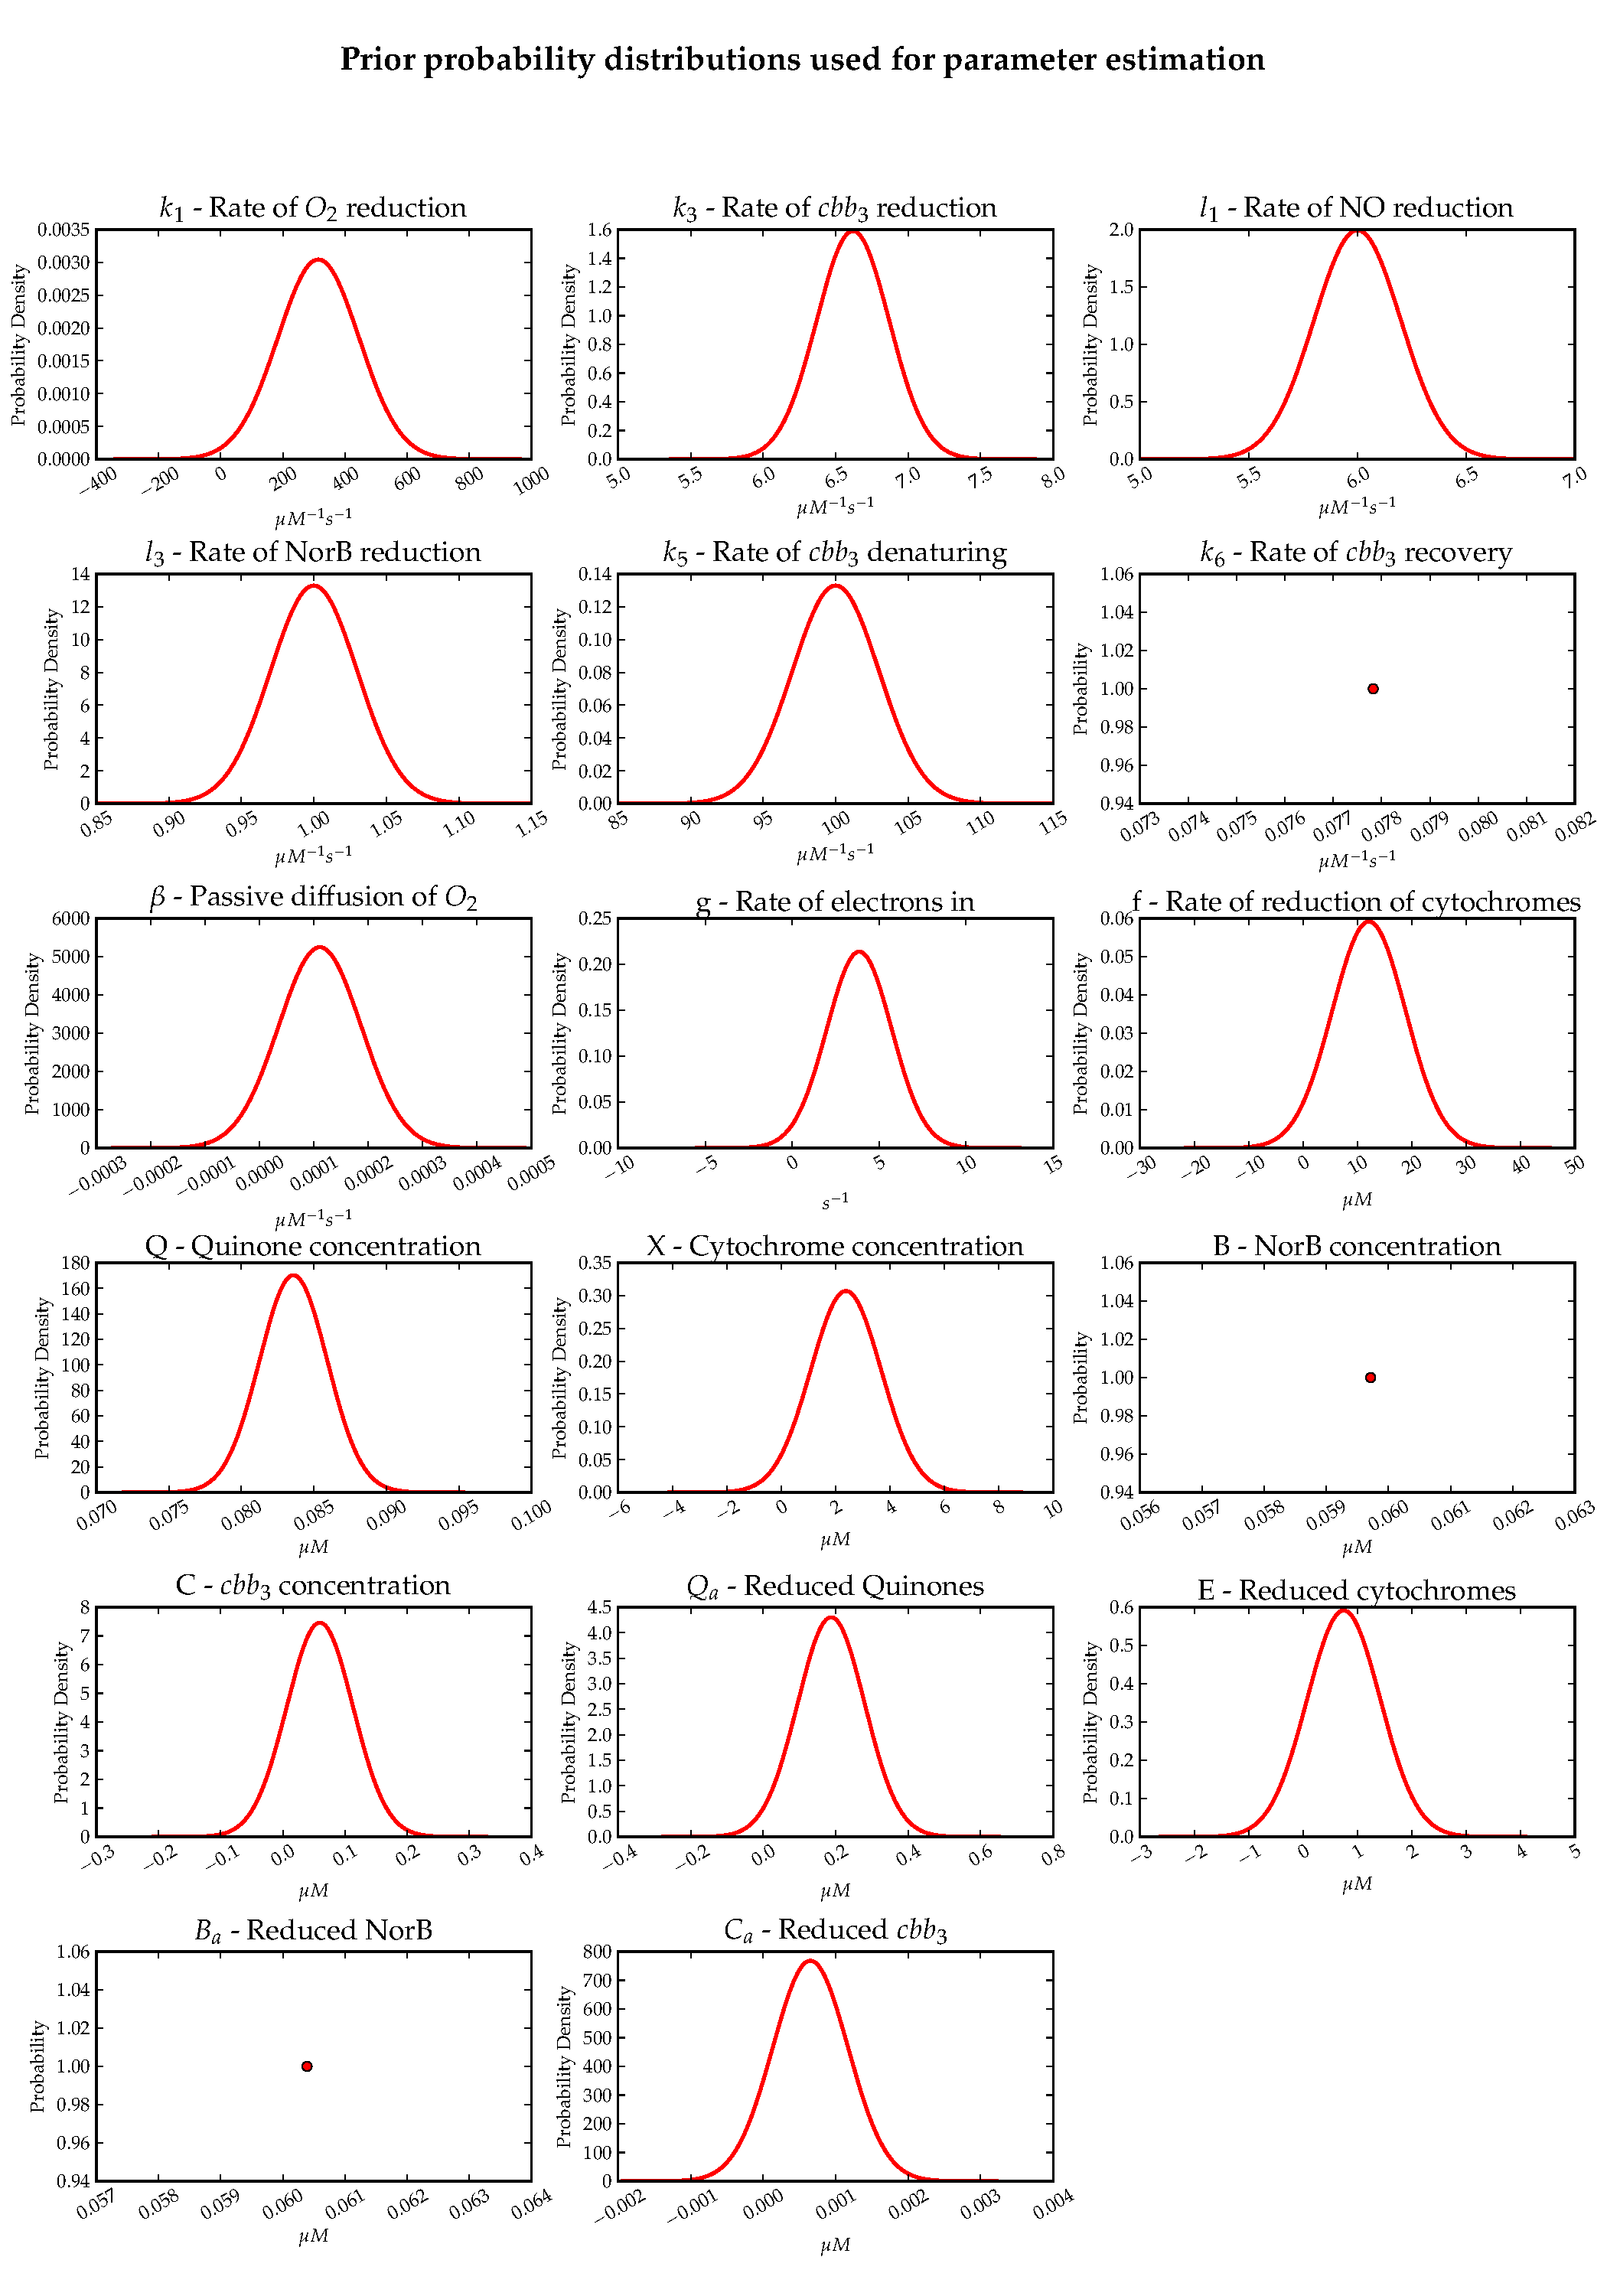
\includegraphics[width=15cm, trim=0cm 0cm 0cm 0cm]{./06-noreduction/data/aer-no-priors.pdf}
 % priors.pdf: 1008x1008 pixel, 72dpi, 35.56x35.56 cm, bb=0 0 1008 1008
 \caption[Prior probability distributions for aerobic nitric oxide reduction]{{\bf Prior probability distributions for aerobic nitric oxide reduction}. These are the probability distributions used as priors by the parameter estimation algorithm. Where no values were available in the literature, the probability distribution represents a flat prior from 0 to $\infty$ with the initial value being determined by preliminary experiment.
 \label{fig:aer_no_priors}}
\end{figure}

\subsubsection{Parameter Estimation Results}
The parameter estimation procress was run in the same fashion as that described in Chapter \ref{chap:oxygenreduction}. The 3 experimental datasets were run 20 times (each) for 20,000 iterations using the prior probability distributions shown in Figure \ref{fig:aer_no_priors}. A representative example of the solved output from one of the trajectories from the experimental dataset shown in Figure \ref{fig:nodata} is shown in Figure \ref{fig:nosim}. This figure was generated from the set of parameters that produced the most fit output compared to the input dataset.
\begin{figure}[tbp]
 \centering
 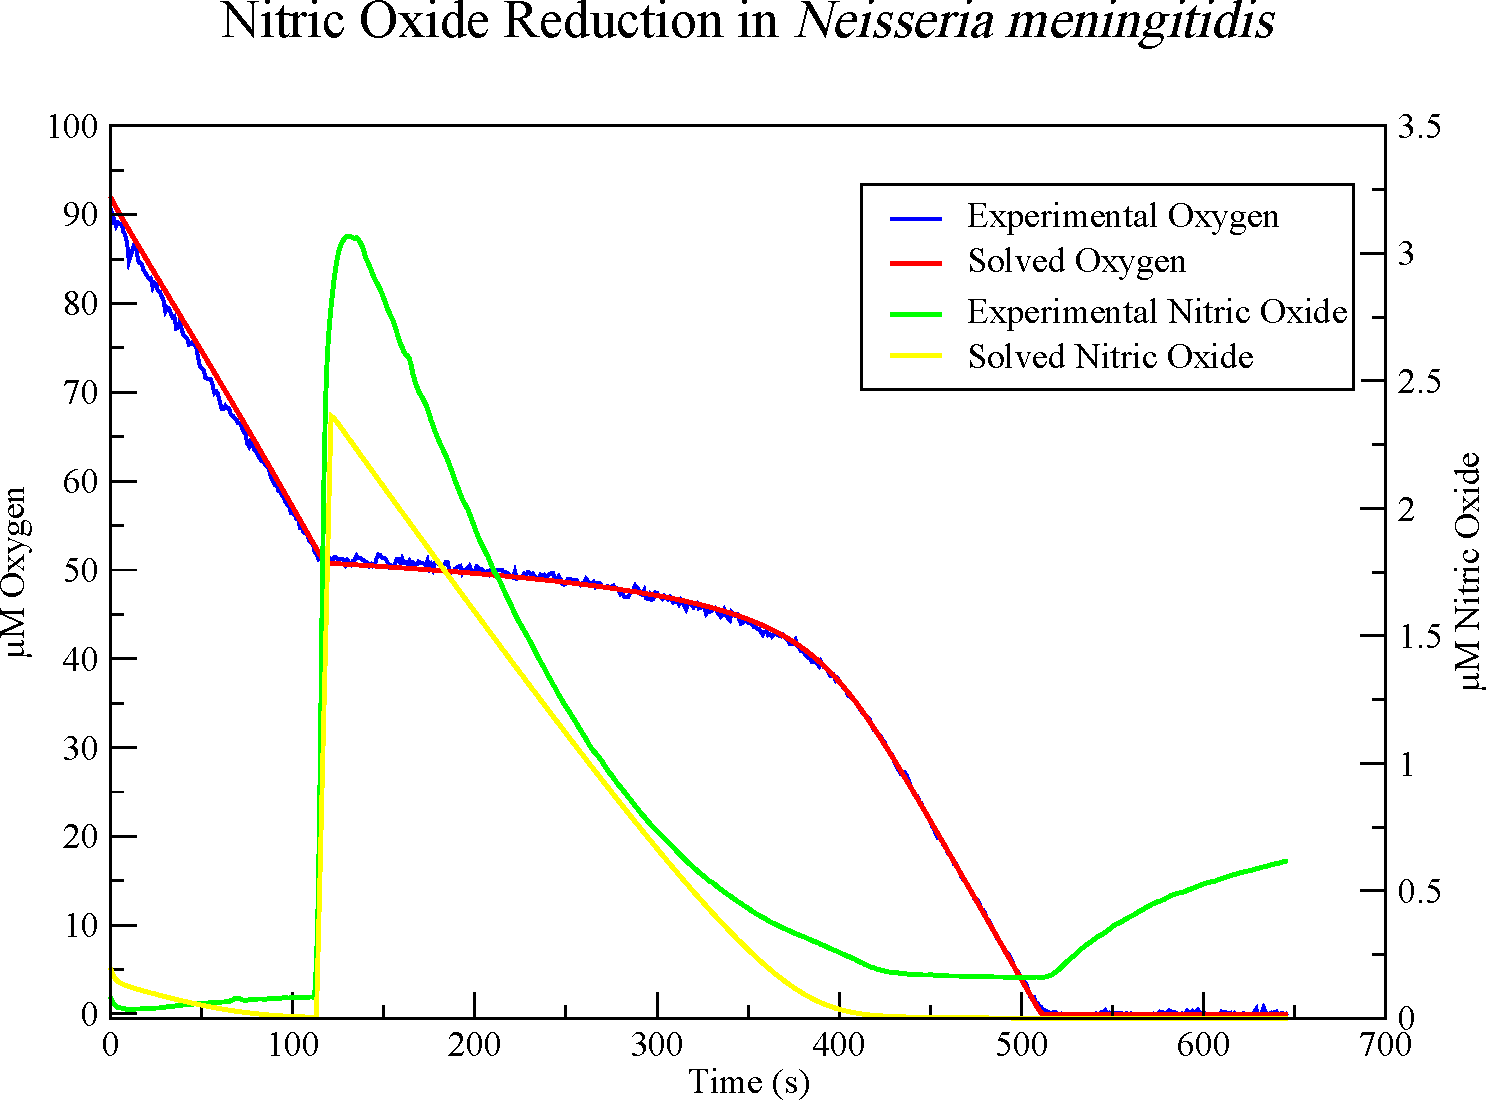
\includegraphics[width=14cm, trim=2cm 1cm 4cm 1cm]{./06-noreduction/data/aer-no-sim.pdf}
 % nosim.eps: 0x0 pixel, 300dpi, 0.00x0.00 cm, bb=0 0 794 595
 \caption[{Nitric Oxide Reduction in \textit{Neisseria meningitidis}.}]{{\bf Nitric Oxide Reduction in \textit{Neisseria meningitidis}.} This dataset shows the effect on rate of oxygen reduction as nitric oxide is introduced to the system. The solved output, using prior probabilities from the oxygen reduction dataset show an almost perfect match to the features of the experimental dataset. The solved oxygen concentrations match the experimental dataset so closely as to be almost invisible.}
 \label{fig:nosim}
\end{figure}
The model was able to generate a parameter set from the prior probability distributions that could accomodate all the new features of the dataset as evidenced by the closeness of fit of the solved output to the experimental data. This parameter set will also still be able to model simple oxygen reduction.
\subsubsection{Analysis of Convergence}
\subsubsection{Analysis of Correlation}
\subsection{Discussion}
\section{Microaerobic Nitric Oxide Reduction}
\subsection{Introduction}
\subsection{Results}
\subsection{Discussion}
\section{\texorpdfstring{Aerobic Nitric Oxide Reduction in \textit{nsrR$^\textrm{-}$} mutant}{Aerobic Nitric Oxide Reduction in nsrR- mutant}}
\subsection{Introduction}
 The $\mathit{nsrR}^-$ mutant, which expresses NorB in an essentially constitutive manner was not effective in generating a usable dataset as it removed any NO almost instantaneously resulting in an almost featureless dataset (data not shown).
\subsection{Results}
\subsection{Discussion}